% !TeX program = pdflatex
% The per-voice Fourier signature: the bass is the spectrally purest voice.
% Author: Carles Marin (with Claude, Anthropic, as AI assistant).
% Style: first-tier mathematical-music-theory note -- restrained, question-driven, a developing narrative
% with a historical thread; booktabs tables with sparing semantic spot color (grayscale-readable);
% one-column serif. Note #4 in the music-math series (companion to phase_taxonomy_note.tex).
% Build: pdflatex per_voice_note.tex (twice, for refs).  Figures: figs/*.pdf ; audio: media/*.
% Source of record: research/music-math/per_voice_signature.md (Curiosity, private repo).

\documentclass[11pt]{article}
\usepackage[T1]{fontenc}
\usepackage{lmodern}
\usepackage{amsmath,amssymb,amsthm,booktabs,graphicx}
\usepackage[hidelinks]{hyperref}
\usepackage{xurl}
\usepackage[table]{xcolor}
\usepackage[margin=1in]{geometry}
\usepackage{microtype}
\usepackage{float}
\usepackage{placeins}
\usepackage{tikz}
\usetikzlibrary{arrows.meta,positioning,calc}
% two semantic spot colors (meaning is ALSO carried by weight, so tables read in grayscale)
\definecolor{ctA}{HTML}{1B6F8C} % the "structural / pure" accent
\definecolor{ctB}{HTML}{B5530F} % the "chromatic / colour" accent
\setlength{\emergencystretch}{2em}
% float placement -- pack floats onto text pages, minimise white gaps
\renewcommand{\topfraction}{0.92}
\renewcommand{\bottomfraction}{0.85}
\renewcommand{\textfraction}{0.08}
\renewcommand{\floatpagefraction}{0.75}
\setcounter{topnumber}{3}
\setcounter{bottomnumber}{2}
\setcounter{totalnumber}{4}
\raggedbottom % collect vertical slack cleanly at page bottoms instead of stretching mid-page
\newtheorem{theorem}{Theorem}
\newtheorem{proposition}{Proposition}
\newtheorem{lemma}{Lemma}
\newtheorem{remark}{Remark}
\newcommand{\lean}[1]{\texttt{#1}}
\newcommand{\Ztwelve}{\mathbb{Z}_{12}}
\newcommand{\Zn}[1]{\mathbb{Z}_{#1}}
\newcommand{\Ahat}{\hat{A}}
% a light "question" lead-in for each section (the connecting thread)
\newcommand{\question}[1]{\smallskip\noindent\textit{#1}\smallskip}
% per-file audio links (live on the public repo); shown in accent color so they read as clickable
\newcommand{\audiobase}{https://github.com/karlesmarin/music-math/raw/main/media}
\newcommand{\audio}[1]{\href{\audiobase/#1}{\textcolor{ctA}{\footnotesize\,[$\flat$\,audio]}}}

\title{\bf The per-voice Fourier signature:\\ the bass is the spectrally purest voice}
\author{Carles Mar\'in\thanks{Prepared with the assistance of an AI system (Claude, Anthropic).
The mathematics is classical and the central finding is empirical; every claim, scope statement, and
limitation is the author's responsibility. The boundary of the contribution is stated plainly in
Section~\ref{sec:novelty}, and the Lean~4 kernel---not the assistant---is what certifies the formalized
part (Section~\ref{sec:checked}).}\\[3pt]
  \normalsize Independent researcher\\
  \normalsize \texttt{karlesmarin@gmail.com}}
\date{June 2026\\[3pt]\normalsize DOI: \href{https://doi.org/10.5281/zenodo.20971090}{10.5281/zenodo.20971090}
\quad\textbullet\quad \href{https://github.com/karlesmarin/music-math}{github.com/karlesmarin/music-math}}

\begin{document}
\maketitle

\begin{abstract}\noindent
For three centuries music theory has held that the bass is special---the \emph{basse fondamentale} of
Rameau, the figured-bass tradition, Riemann's harmonic functions: the lowest voice carries the harmonic
roots, the foundation. That has always been a \emph{structural} claim. The discrete Fourier transform of
pitch-class distributions (Lewin, Quinn, Amiot, Yust) turned chord ``qualities'' into numbers---the
magnitude $|a_k|$ of the $k$-th coefficient measures a character: $|a_5|$ diatonicity, $|a_1|$
chromaticity, $|a_6|$ whole-toneness. That program reads a piece by \emph{time}; it has never asked whether
each \emph{voice} carries a different spectral fingerprint. We do. Over $334$ four-part Bach chorales the
naive guess---that the fifth-walking bass is the most diatonic ($|a_5|$) voice---is \emph{false} (the
soprano is). But the data shows something sharper: the \textbf{bass is the spectrally purest voice}, lowest
in chromaticity ($\alpha_1=|a_1|/|a_0|$, paired $t=-20$) and whole-toneness ($\alpha_6$, $t=-15$),
\emph{despite using the widest pitch-class vocabulary}---so this is not a cardinality artifact. The cause is
\textbf{root realization} acting through two channels: functional roots move by fifths/fourths (odd
intervals), which balance even/odd pitch-class weight and drive $\alpha_6\!\to\!0$ (the \emph{parity}
channel), and the bass's wide tessitura spreads its weight around the chromatic circle, lowering $\alpha_1$
(the \emph{dispersion} channel). The effect is \textbf{texture-bounded}: strong in functional-bass
homophony (Bach chorales; Palestrina), it fades in imitative (Monteverdi madrigals) and pre-functional
(Trecento) textures---so the signature is a \emph{diagnostic of functional-bass writing}, and the boundary
confirms the mechanism. The parity channel's kernel---$a_6$ equals the even-minus-odd pitch-class
parity---is machine-checked in Lean~4 (\lean{ParityA6.lean}, sorry-free, axiom-clean, general even
universe). Every ingredient is classical (Rameau/Riemann's functional bass; $a_6=$ pc-parity, Amiot;
the single-note-move rule, Hoffman); the contribution is the \textbf{per-voice magnitude law}---a measured,
explained, certified, and honestly bounded fact---not new mathematics.
\end{abstract}

\section{Is the bass really the foundation?}\label{sec:hook}

When Jean-Philippe Rameau placed the \emph{basse fondamentale} at the centre of harmony in
1722~\cite{Rameau}, he made precise an old practical instinct: the lowest voice is not just another melody
but the bearer of the chord roots, the ground on which harmony stands. The figured-bass tradition encoded
the same priority, and Hugo Riemann's harmonic functions~\cite{Riemann} later read tonal motion as a logic
of bass-rooted functions. ``The bass is the foundation'' became one of the most durable claims in music
theory---and it stayed a \emph{structural}, qualitative one.

That instinct was, for a century and a half, also a daily practice. In the Baroque \emph{basso continuo}, a
single bass line---annotated with figures---was enough for a keyboardist to realize an entire harmony, the
upper voices following from the bass rather than the other way round. Rameau's \emph{basse fondamentale}
gave the practice a theory: beneath the sounding bass lies a conceptual line of chord \emph{roots}, and
harmony is the motion of that line; Riemann later recast the same motion as a compact grammar of tonic,
subdominant and dominant functions, again anchored below. Across the common-practice era the bass was thus
singled out three times over---in performance, in theory, and in pedagogy---as the voice that
\emph{defines} the harmony. The claim was everywhere; a number for it was nowhere.

Two and a half centuries after Rameau, David Lewin~\cite{Lewin1959}---in a two-page note of 1959 that is
now seen as the seed of the whole subject---began to turn the internal structure of chords into Fourier
coefficients, an idea revived by Ian Quinn as a theory of chord ``quality''~\cite{Quinn} and built into a
discipline by Emmanuel Amiot~\cite{Amiot} and Jason Yust~\cite{Yust2017,Yust2019}. Encode a chord or a passage as a distribution
on the twelve pitch classes $\Ztwelve$, take its discrete Fourier transform, and the \emph{magnitudes}
$|a_k|$ read as musical \textbf{characters}: $|a_5|$ is diatonicity, $|a_4|$ octatonicity, $|a_6|$
whole-toneness, $|a_1|$ chromaticity, and so on. The character profile of a piece can be tracked, charted,
even drawn as a pie. But every analysis in this program segments a texture by \emph{time}---sliding windows
over the whole-texture pitch-class distribution. \textbf{None has asked the orthogonal question: does each
voice, by its registral role, carry a different Fourier character profile?}

This note follows that one question. It lets us put Rameau's structural intuition on a measuring
instrument: if the bass really is the harmonic foundation, it should leave a measurable spectral
\emph{fingerprint}, distinct from the voices above it. It does---but not the fingerprint one would first
guess, and only exactly where harmony is functional.

\section{Setup: the per-voice DFT}\label{sec:setup}

Fix a voice $v$ in a piece and form its \textbf{duration-weighted pitch-class distribution}
$\mu_v:\Ztwelve\to\mathbb{R}_{\ge 0}$, where $\mu_v(x)$ is the total sounding duration the voice spends on
pitch class $x$ (octave collapsed). Its discrete Fourier transform is
\[
  a_k(v)\;=\;\hat\mu_v(k)\;=\;\sum_{x\in\Ztwelve}\mu_v(x)\,e^{-2\pi i\,kx/12},\qquad k=0,1,\dots,6,
\]
with $a_0=$ total weight. We compare voices by the \textbf{normalized character}
$\alpha_k(v)=|a_k(v)|/|a_0(v)|\in[0,1]$, which is invariant to how loud or long the voice is. The named
characters are the standard ones~\cite{Amiot,Yust2019}: $\alpha_1$ chromatic, $\alpha_2$ quartal,
$\alpha_3$ augmented, $\alpha_4$ octatonic, $\alpha_5$ diatonic, $\alpha_6$ whole-tone. Voices are
identified by \emph{register} (mean pitch), so ``bass'' means the lowest-sounding part, ``soprano'' the
highest---no reliance on part names. The whole construction is linear in the voice decomposition; the
contribution here is empirical, in what the measurement reveals.

\section{The first guess, and the surprise}\label{sec:law}

\question{P\textsubscript{1}. The bass walks by fifths and carries the roots---so is it the most
fifth-generated, i.e.\ the most \emph{diatonic} ($\alpha_5$), voice?}

It is a natural guess, and it is \textbf{wrong}. Over the $334$ four-part chorales of J.S.~Bach
(\lean{music21} corpus), the soprano is the most diatonic voice ($\alpha_5=0.580$ vs the bass's $0.535$,
paired $t=-10.4$). The bass is not where diatonicity peaks.

What the measurement \emph{does} reveal is sharper and more robust. The bass is the \textbf{spectrally
purest} voice: it is the lowest in chromaticity $\alpha_1$ and the lowest in whole-toneness $\alpha_6$, by
a wide margin (Figure~\ref{fig:camembert}, Table is Figure~\ref{fig:heatmap}). Per-voice means, Bach:

\begin{center}\small
\begin{tabular}{@{}lcccccc@{}}
\toprule
\textbf{voice} & $\alpha_1$ chrom & $\alpha_2$ & $\alpha_3$ & $\alpha_4$ oct & $\alpha_5$ diat & $\alpha_6$ w-tone\\
\midrule
Bass    & \textbf{0.130} & 0.207 & 0.257 & 0.118 & 0.535 & \textbf{0.079}\\
Tenor   & 0.279 & 0.181 & 0.261 & 0.186 & 0.525 & 0.190\\
Alto    & 0.363 & 0.233 & 0.298 & 0.197 & 0.505 & 0.223\\
Soprano & 0.297 & 0.170 & 0.233 & 0.183 & \textbf{0.580} & 0.216\\
\bottomrule
\end{tabular}
\end{center}

Paired against the soprano: $\alpha_1$ $t=-20.3$, $\alpha_6$ $t=-14.8$---the two largest effects in the
table. \textbf{The bass is the least chromatic and least whole-tone voice; the soprano is the most
diatonic; the inner voices are the most chromatic.} One can hear the contrast: the bass of a chorale soloed
\audio{bwv66_6_bass.wav} against its alto \audio{bwv66_6_alto.wav}.

\begin{figure}[H]\centering
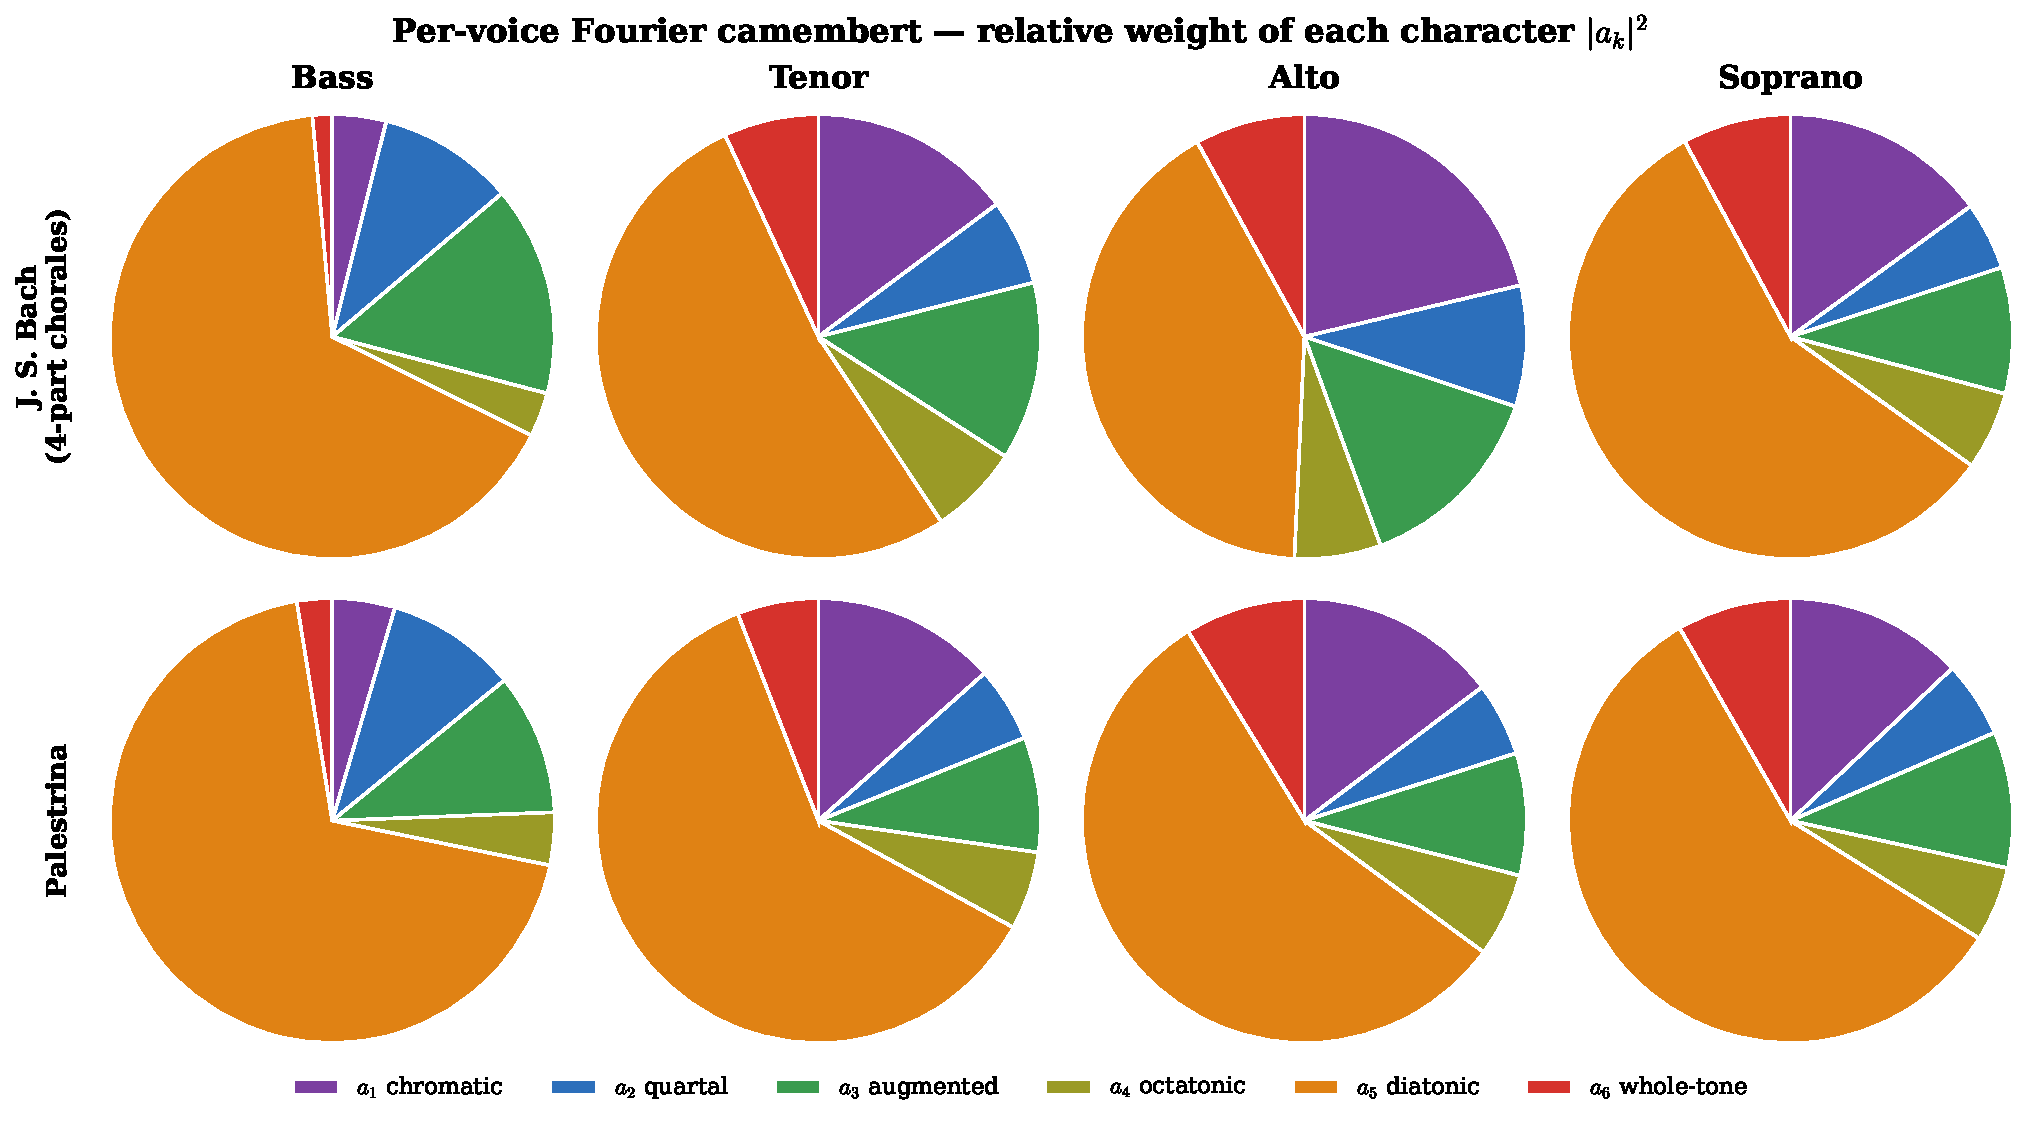
\includegraphics[width=\linewidth]{figs/fig1_camembert.pdf}
\caption{The per-voice Fourier ``camembert'': the relative weight of each character ($|a_k|^2$, Parseval)
for Bass/Tenor/Alto/Soprano, in Bach chorales (top) and Palestrina (bottom). The \textbf{bass pie} is
visibly thin in the chromatic (purple) and whole-tone (red) slices and fat in diatonic (orange); the
\textbf{alto} carries the largest chromatic wedge. The signature is legible at a glance and reproduces
across two corpora two centuries apart.}
\label{fig:camembert}
\end{figure}

\paragraph{Not a cardinality artifact.} A spread-out distribution has small high-$k$ coefficients, so one
might suspect the bass simply uses fewer pitch classes. The opposite is true: the bass uses
\emph{more} distinct pitch classes than the soprano ($9.5$ vs $7.5$ on average) and has higher entropy,
yet has the lowest $\alpha_1$. The low chromaticity is genuine distributional structure, not a counting
effect.

\begin{figure}[H]\centering
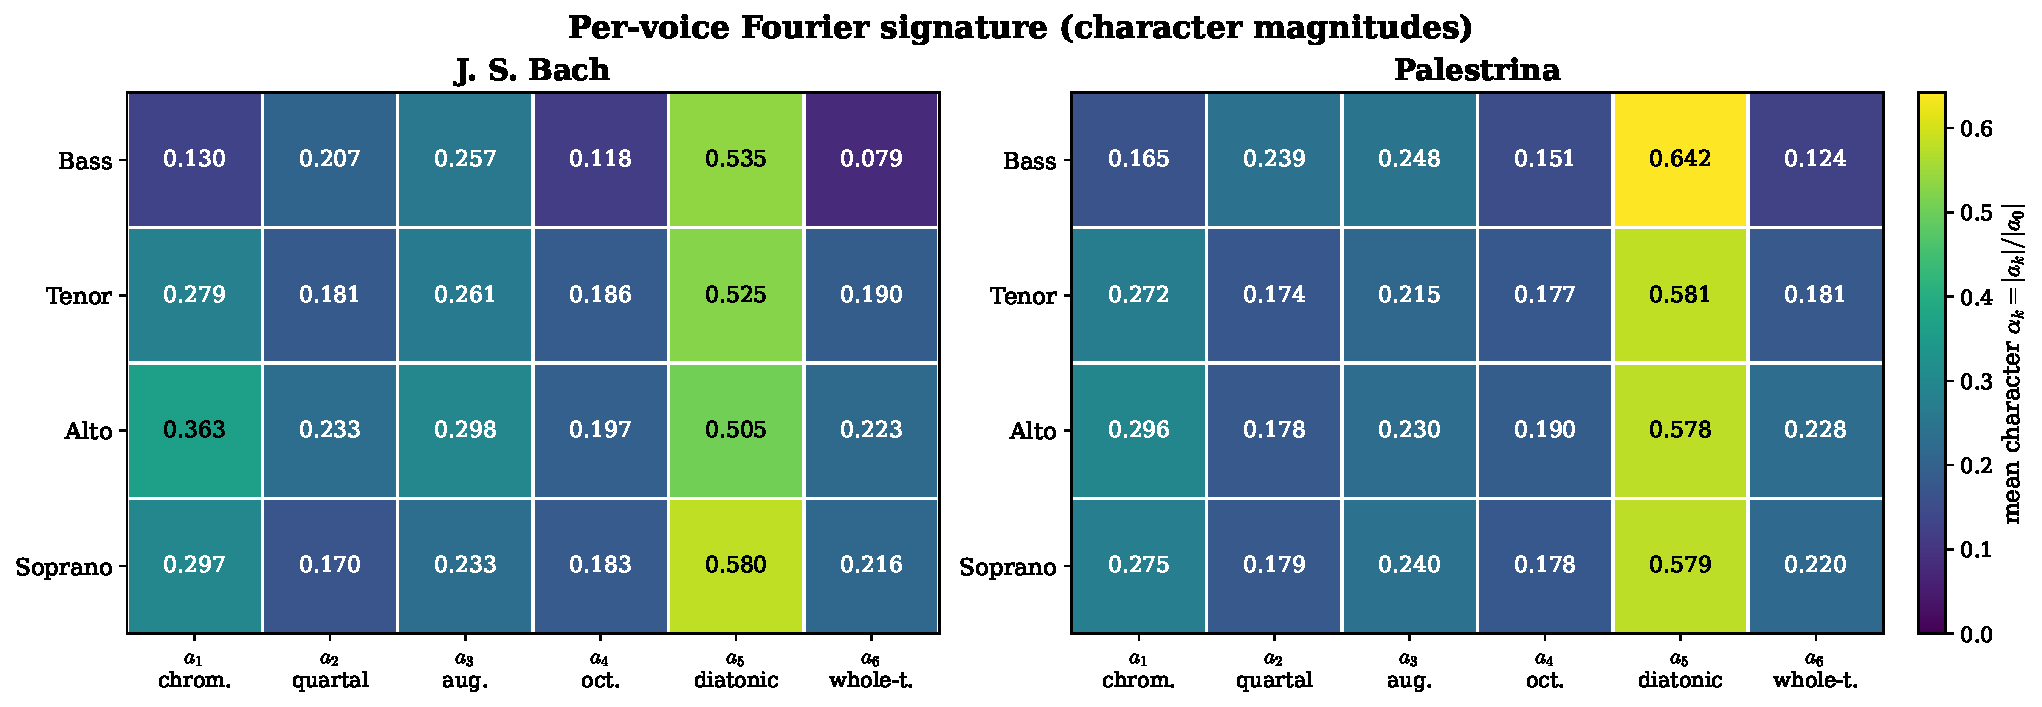
\includegraphics[width=\linewidth]{figs/fig7_heatmap.pdf}
\caption{The whole signature as a matrix: voices $\times$ characters $\alpha_k$, Bach and Palestrina. The
\textbf{bass row} is darkest in $a_1$ and $a_6$ and brightest in $a_5$, in both corpora; the
\textbf{alto} is brightest in $a_1$. The diatonic column dominates every voice (tonal/modal music), but the
\emph{contrast between voices} lives in $a_1$ and $a_6$.}
\label{fig:heatmap}
\end{figure}

\section{Why: root realization, in two channels}\label{sec:why}

\question{P\textsubscript{2}. Why is the bass spectrally pure---and why in $a_1$ and $a_6$ specifically?}

Because, to $95\%$ cosine fidelity (duration-weighted, Bach), the bass distribution \emph{is} the
chord-root distribution: the bass realizes the harmonic roots. Functional root motion proceeds by
fifths and fourths---intervals $7$ and $5$, both \textbf{odd}. This single fact drives two distinct
spectral channels.

\paragraph{The parity channel ($a_6$).} The whole-tone coefficient is, exactly,
$a_6=\sum_{x}\mu(x)\,(-1)^x=(\text{even-pc weight})-(\text{odd-pc weight})$: it reads the even/odd
\textbf{parity imbalance} of the distribution (this identity is the certified kernel of
Section~\ref{sec:checked}). An odd interval flips pitch-class parity; a root progression that walks by
fifths therefore alternates parity and \emph{balances} the two whole-tone collections, sending
$a_6\to0$\,\audio{arch_wholetone_highA6.wav}. Empirically, the correlation of $\alpha_6$ with the voice's odd-interval fraction is $-0.49$:
the more a voice moves by odd intervals (the bass most of all), the lower its whole-toneness.

\paragraph{The dispersion channel ($a_1$).} The coefficient $a_1$ measures chromatic \emph{clustering}---it
is large when weight piles up in a contiguous arc of the chromatic circle. The functional bass leaps; it
spans the widest tessitura of the four voices ($\approx 18$ semitones vs $\approx 12$), so its
pitch-class weight is spread widely around the circle rather than clustered, and $\alpha_1$ is
low\,\audio{arch_fifthchain_lowA1A6.wav}.
Empirically, the correlation of $\alpha_1$ with voice range is $-0.67$. Figure~\ref{fig:pcclock} shows this
directly: the bass's weight fans out around the clock, the alto's bunches into an arc.

\begin{figure}[H]\centering
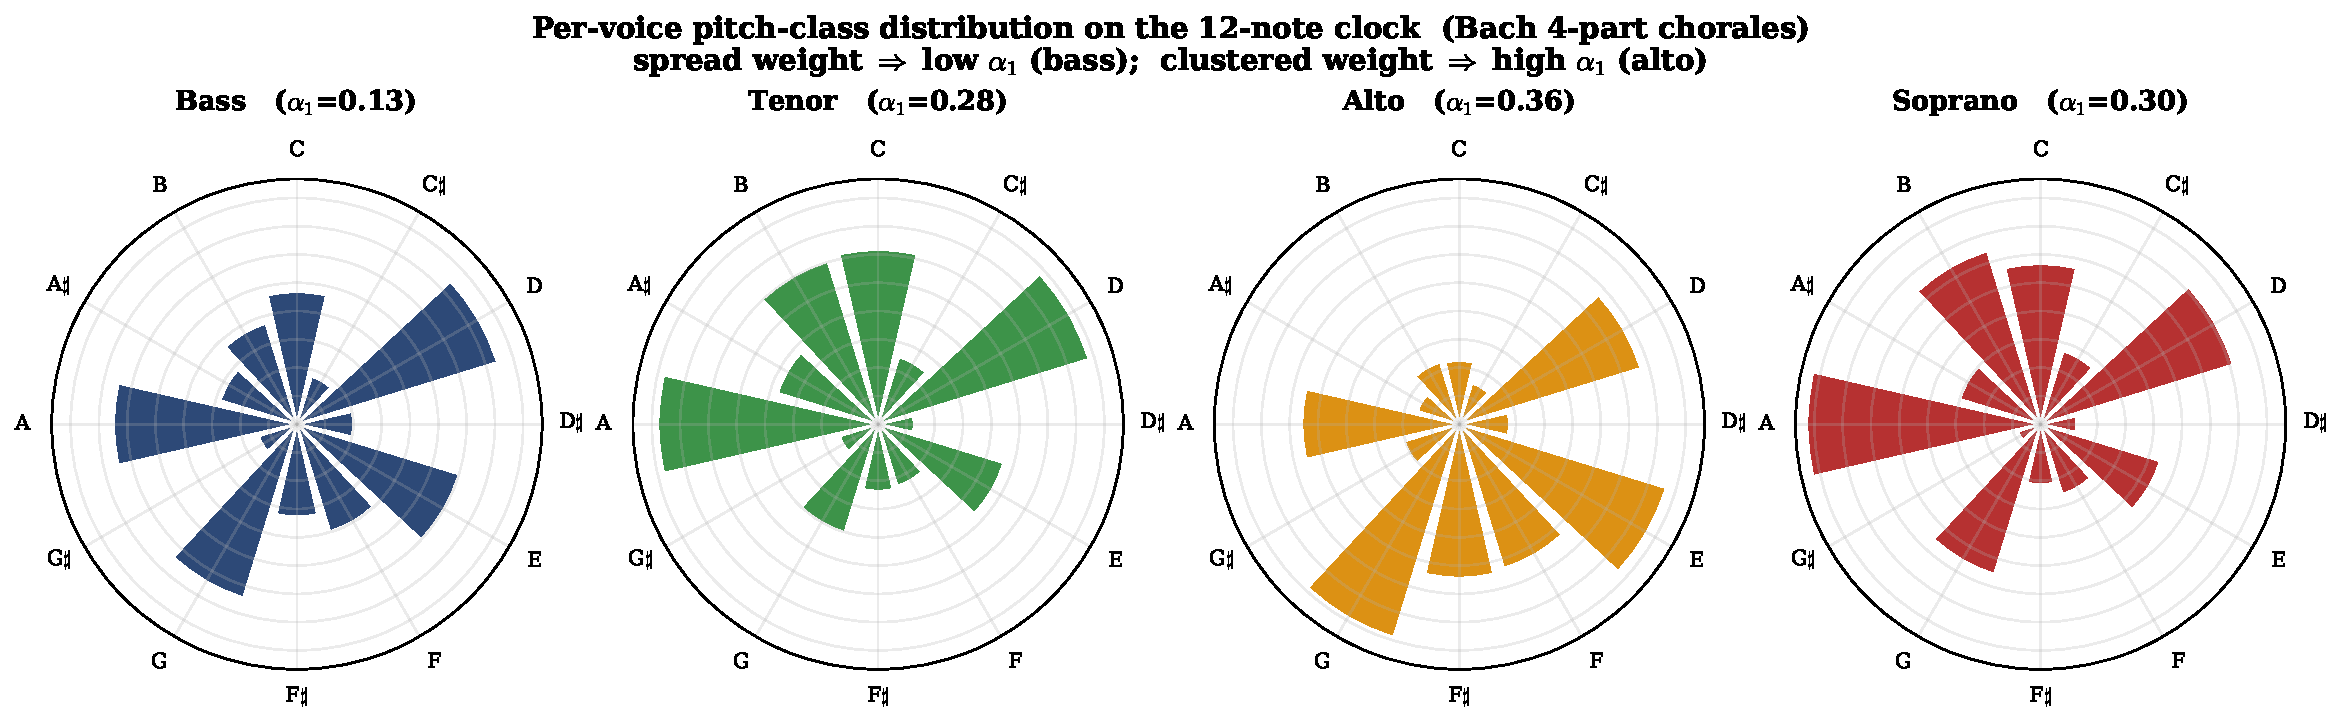
\includegraphics[width=\linewidth]{figs/fig5_pc_clock.pdf}
\caption{The per-voice pitch-class distribution drawn on the twelve-note clock (Bach). The \textbf{bass}
($\alpha_1=0.13$) spreads its weight widely around the circle (low chromatic clustering); the
\textbf{alto} ($\alpha_1=0.36$) bunches into a narrow arc (high clustering). Spread weight $\Rightarrow$
low $a_1$; clustered weight $\Rightarrow$ high $a_1$---the dispersion channel, seen.}
\label{fig:pcclock}
\end{figure}

\paragraph{A mechanism that was \emph{not} the cause.} It is tempting to attribute the bass's low
chromaticity to its melodic motion---``the bass avoids semitone steps.'' It does not: the correlation of
$\alpha_1$ with the fraction of semitone melodic steps is just $+0.01$, and the bass has as many
semitone steps as the other voices. The cause is in the pitch-class \emph{distribution} (which classes,
how spread), not in the melodic surface. We record the refuted mechanism because it sharpens the true one.

\section{The historical sweep: a diagnostic of functional-bass texture}\label{sec:history}

\question{P\textsubscript{3}. If the cause is the functional bass, the law should appear exactly where the
bass bears roots---and fade where it does not. Does it?}

It does---and the cleanest way to see it is to walk four corpora across four centuries, each embodying a
different relationship between the lowest voice and the harmony. In the Italian \textbf{Trecento} (the
fourteenth-century \emph{Ars Nova} of Landini and his contemporaries) polyphony is built line by line above
a structural \emph{tenor}; the lowest sounding voice is not yet a bearer of harmonic roots, and the
signature is simply absent ($\alpha_1$ bass-purer-than-top in $52\%$ of works, $\alpha_6$ in $58\%$---no
better than the $50\%$ coin toss). By Palestrina's \textbf{stile antico} (sixteenth-century modal
counterpoint, the music of the Counter-Reformation) a clear lowest voice already governs the harmonic
implication of each sonority, and the signature is strong ($87\%$, $77\%$). It is strong again two
centuries later in \textbf{Bach}'s chorales ($85\%$, $73\%$)---the apotheosis of functional four-part
harmony, where the bass simply \emph{is} the figured-bass foundation of \S\ref{sec:hook}. The telling case
is \textbf{Monteverdi}: his madrigals \emph{postdate} Palestrina, yet show the \emph{weaker} effect
($65\%$, $53\%$---near chance), because the expressive \emph{seconda prattica} madrigal is imitative and
text-driven, scattering its chromatic colour across five near-equal voices in which no single line is the
privileged root-bearer. So the signature tracks \textbf{texture, not date} (Figure~\ref{fig:sweep}): it
is strong exactly where the bass realizes roots and fades where it does not. The boundary is not a failure
of the law but its confirmation---the same root-realization mechanism that predicts the effect predicts
where it must vanish---and it recasts the effect as a \textbf{diagnostic of functional-bass writing}, a
spectral fingerprint of the very practice Rameau theorized.

\begin{figure}[H]\centering
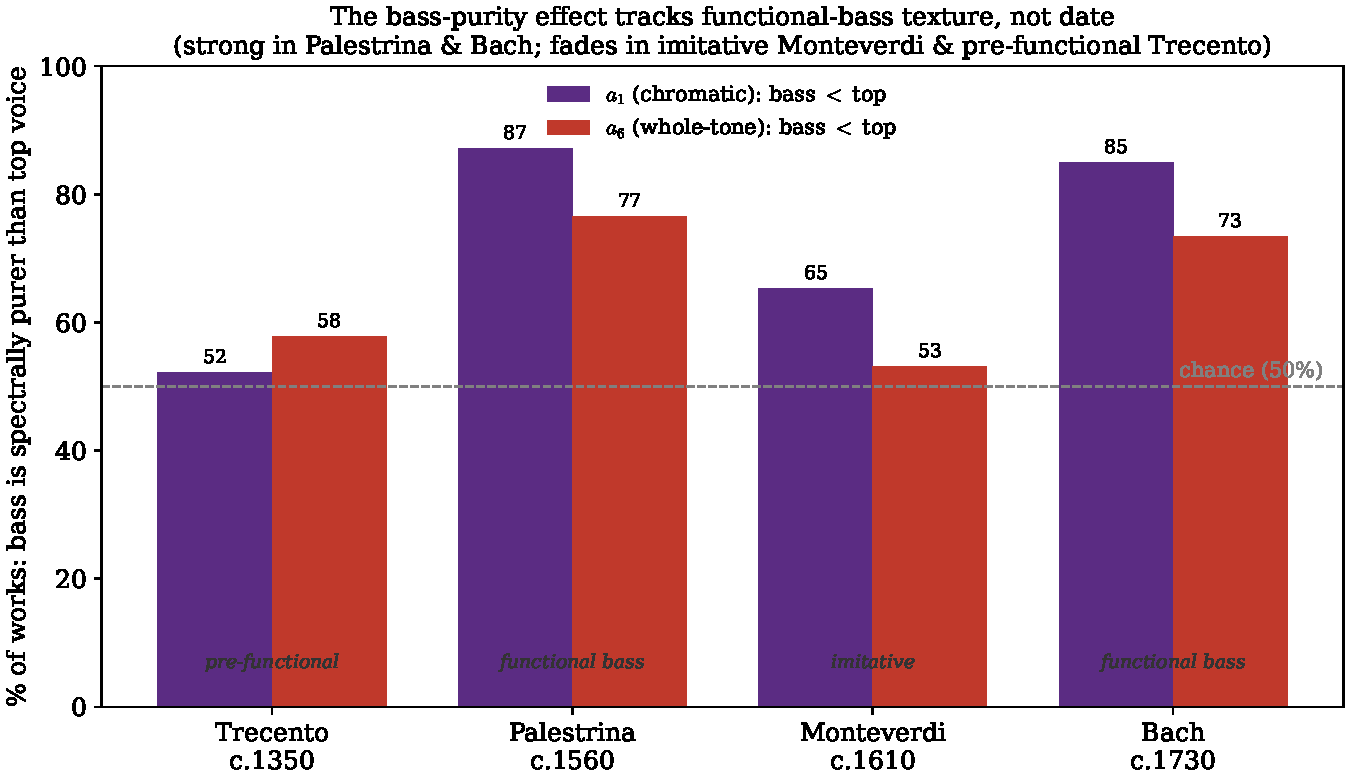
\includegraphics[width=0.92\linewidth]{figs/fig9_historical_sweep.pdf}
\caption{The bass-purity effect across four corpora. Bars: percentage of works in which the bass is
spectrally purer than the top voice, in $a_1$ (chromatic) and $a_6$ (whole-tone), against the $50\%$
chance line. Strong in functional-bass homophony (Palestrina, Bach), it fades in imitative (Monteverdi) and
pre-functional (Trecento) textures---tracking the role of the bass, not chronology.}
\label{fig:sweep}
\end{figure}

\section{The dual: inner voices carry the colour}\label{sec:dual}

\question{P\textsubscript{4}. If the bass is the purest, which voice is the least pure---and why?}

The chromaticity ordering is Bass $0.130<$ Tenor $0.279<$ Soprano $0.297<$ \textbf{Alto $0.363$}: the inner
voices, the alto above all, carry the most chromatic colour\,\audio{arch_chromatic_highA1.wav}. This is the dispersion channel run in reverse:
inner voices occupy the \emph{narrowest} tessitura ($\approx 11$--$12$ semitones), so their weight is
compressed into a chromatic band and $\alpha_1$ is high. It is the registral-spread story, not a
melodic-chromaticism one (the semitone-step correlation is null, as in \S\ref{sec:why}). The four voices
sit, in the diatonic-phase plane $(\Phi_3,\Phi_5)$, almost on top of one another
(Figure~\ref{fig:phaseplane})---they share a key---so the inter-voice information is in the
\emph{magnitudes} $\alpha_1,\alpha_6$, not the phases: a bass and a soprano differ in spectral
\emph{purity}, not in tonal centre.

This inverts the textbook image in a precise way. The \emph{outer} voices are the structural frame---the
bass rooting the harmony, the soprano carrying the tune---while the \emph{inner} voices are where the
chromatic colour lives: the home of suspensions, passing and neighbour tones, and the small chromatic
voice-leading that fills out a four-part texture. That the alto is the single most chromatic voice is thus
the spectral echo of a practice as old as the \emph{altus} of Renaissance polyphony---the inner parts move
by the short, often chromatic steps that the bass, leaping by fifths, never takes, and the soprano, singing
the diatonic melody, mostly avoids. Purity below, tune above, colour within: the Fourier characters recover
the division of labour of the four-voice chorale itself.

\begin{figure}[H]\centering
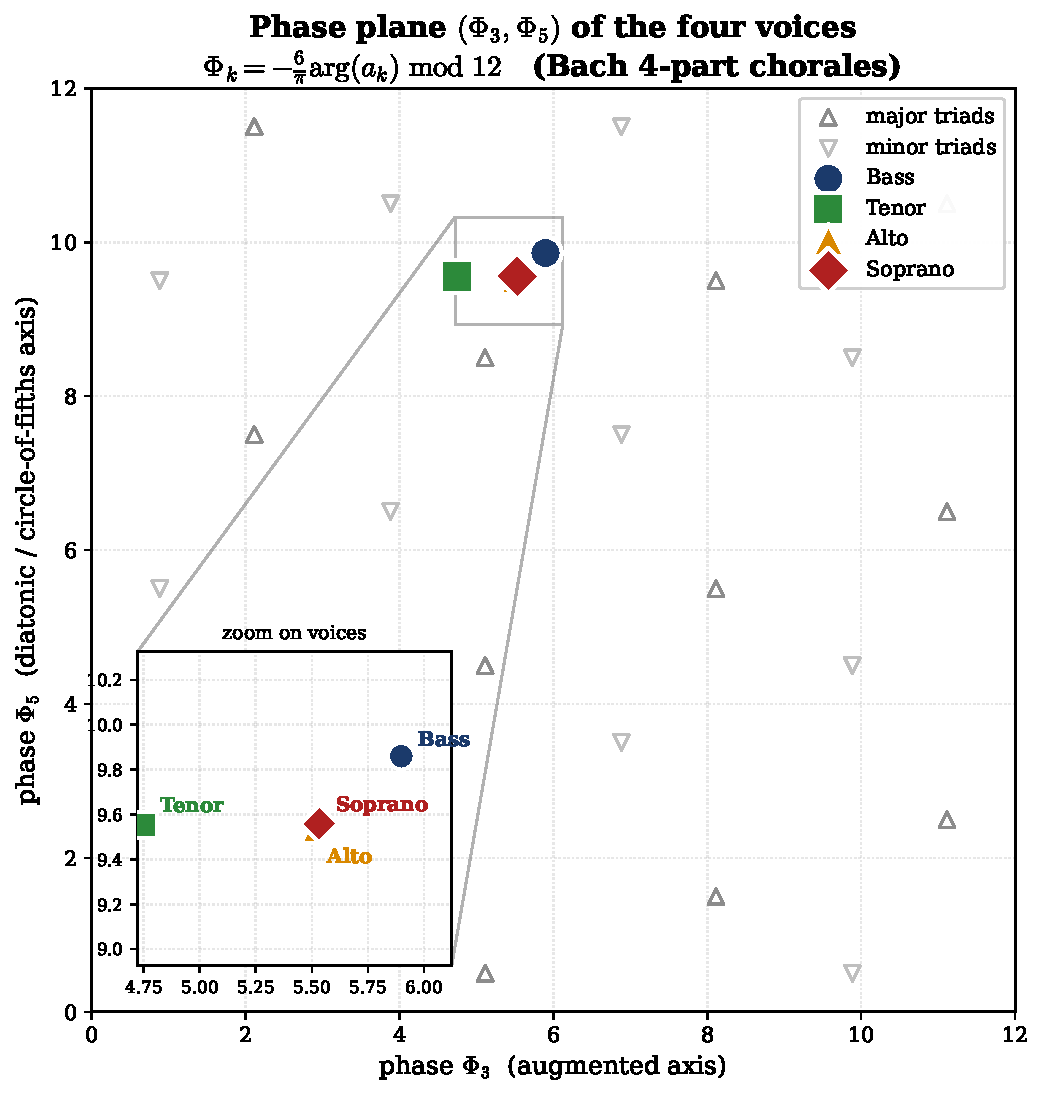
\includegraphics[width=0.50\linewidth]{figs/fig6_phase_plane.pdf}
\caption{The four voices in the diatonic phase plane $(\Phi_3,\Phi_5)$ against the $24$ major/minor triads.
The voices are near-coincident (a shared key): the per-voice contrast is carried by the character
\emph{magnitudes} ($a_1,a_6$), not the phases.}
\label{fig:phaseplane}
\end{figure}

\section{What is machine-checked}\label{sec:checked}

\question{P\textsubscript{5}. The empirical law rests on a measurement; what part of it is certified?}

The parity channel's kernel---the identity that makes the whole-tone coefficient a parity count---is proved
in Lean~4 (\lean{ParityA6.lean}, namespace \lean{ParityA6}, sorry-free; built on the project's
\lean{Fourier.lean}). Table~\ref{tab:lean} lists the results. The headline is that $a_6$ \emph{is} the
even-minus-odd parity imbalance, with the order-$2$ frequency reading parity in \emph{any} even universe
$\Zn{2m}$, not only $\Ztwelve$. The axiom audit (\lean{\#print axioms}) returns at most
\lean{[propext, Classical.choice, Quot.sound]} on every named result---no \lean{sorryAx}, no
\lean{Lean.ofReduceBool}---confirmed by recompiling in the project's fast-loop environment (EXIT~0).

\begin{table}[H]
\centering\small
\rowcolors{2}{ctA!7}{white}
\begin{tabular}{@{}l p{0.58\textwidth}@{}}
\toprule
\rowcolor{ctA!22}
\textbf{Lean result (\lean{ParityA6.lean})} & \textbf{Statement}\\
\midrule
\lean{Ahat\_six\_eq\_sum\_neg\_one\_pow} & $\Ahat(6)=\sum_{x\in A}(-1)^{x}$ --- the whole-tone coefficient is the signed parity sum.\\
\lean{Ahat\_six\_eq\_card\_sub} & $\Ahat(6)=\#(\text{even pcs})-\#(\text{odd pcs})$ --- the parity imbalance, over $\mathbb{C}$.\\
\lean{Ahat\_six\_eq\_zero\_iff} & $\Ahat(6)=0\iff \#(\text{even})=\#(\text{odd})$ --- $a_6$ vanishes exactly at even/odd balance.\\
\lean{dftN\_half\_eq\_sum\_neg\_one\_pow} & General even universe: in $\Zn{2m}$, the order-$2$ frequency reads parity, $\hat\mu(m)=\sum_x(-1)^{x}$.\\
\bottomrule
\end{tabular}
\caption{The parity kernel of the $a_6$ channel, machine-checked. Four \lean{example} witnesses accompany
it (C major $a_6=1$; whole-tone $a_6=6$; diatonic $a_6=-1$; a balanced tetrachord $a_6=0$). The math is
classical (see \S\ref{sec:novelty}); this is its first formalization.}
\label{tab:lean}
\end{table}

\section{Novelty, scope, and what this note does not claim}\label{sec:novelty}

\paragraph{Contribution, stated plainly.} This is an \textbf{empirical} note with a \textbf{formalized
kernel}, not new mathematics. Every explanatory ingredient is classical: the functional bass is
Rameau~\cite{Rameau} and Riemann~\cite{Riemann}; the DFT-of-pitch-class-distributions program and the
character readings ($a_5=$ diatonicity, etc.) are Lewin~\cite{Lewin1959}, Quinn~\cite{Quinn},
Amiot~\cite{Amiot}, Yust~\cite{Yust2017,Yust2019}; the identity $a_6=$ pitch-class parity is Amiot
(\emph{The Torii of Phases}~\cite{Torii}, ``$a_6$ takes only two values, depending on the number of odd
pitches''), and the single-note-move mechanism behind it is Hoffman~\cite{Hoffman}. \textbf{The new content
is the per-voice magnitude law}: that, in functional-bass textures, the bass is the spectrally purest voice
(lowest $\alpha_1,\alpha_6$), measured across corpora, explained by root realization in two channels, and
bounded by texture. The DFT program reads textures by \emph{time}; the per-voice (registral) magnitude
contrast is the orthogonal cut, and it is, to our search, unstated.

\paragraph{What this note does \emph{not} claim.}
\begin{itemize}\itemsep2pt
  \item \textbf{Not a theorem.} The law is an empirical regularity; its mathematical kernel is the linearity
        of the DFT over the voice decomposition. Only the parity identity (Table~\ref{tab:lean}) is a Lean
        theorem.
  \item \textbf{Not universal.} The signature is a diagnostic of \emph{functional-bass} texture: strong in
        Palestrina and Bach, weak/absent in Monteverdi madrigals and the Trecento (\S\ref{sec:history}).
  \item \textbf{Not the diatonicity guess.} The bass is \emph{not} the most diatonic ($a_5$) voice; that is
        the soprano. The invariant is the bass's low $a_1$ and $a_6$, not high $a_5$.
  \item \textbf{Not a melodic claim.} The low chromaticity is a property of the pitch-class
        \emph{distribution} (dispersion / parity), not of semitone melodic motion (correlation $+0.01$).
  \item \textbf{Not priority over the DFT program.} Lewin, Quinn, Amiot, and Yust each precede this; we
        cite, measure, formalize, and do not supplant. The parity identity is Amiot/Hoffman; our
        \lean{ParityA6.lean} is its first formalization, and it is \emph{distinct} from---not a corollary
        of---Amiot's tritone lemma (which concerns the \emph{odd}-index coefficients).
\end{itemize}

\paragraph{Open frontier.} A larger corpus and more styles would map the texture boundary precisely (where,
quantitatively, does ``functional-bass'' begin?); a per-voice study of the \emph{phases} (rather than
magnitudes) is untouched here; and the dispersion channel invites a clean statement bounding $a_1$ by a
voice's circular spread.

\section*{Data and code availability}
The per-voice measurements (\lean{music21}: $334$ Bach four-part chorales, $367$ Palestrina works, plus the
Monteverdi and Trecento corpora), the figure toolkit (\lean{voice\_figs.py}, regenerating
Figures~\ref{fig:camembert}--\ref{fig:phaseplane} from the corpora), the sonifications
(\lean{media/}), and the Lean source \lean{ParityA6.lean} accompany this note; each Lean result
is checkable by \lean{\#print axioms} and each script is re-runnable.

\begin{thebibliography}{99}
\bibitem{Rameau} J.-Ph. Rameau, \emph{Trait\'e de l'harmonie r\'eduite \`a ses principes naturels},
  Ballard, Paris, 1722.
\bibitem{Riemann} H. Riemann, \emph{Vereinfachte Harmonielehre}, Augener, London, 1893.
\bibitem{Lewin1959} D. Lewin, ``Re: Intervallic relations between two collections of notes,''
  \emph{J. Music Theory} \textbf{3} (1959), no.~2, 298--301.
\bibitem{Quinn} I. Quinn, ``General equal-tempered harmony,'' \emph{Perspectives of New Music}
  \textbf{44}/2--\textbf{45}/1 (2006--2007).
\bibitem{Amiot} E. Amiot, \emph{Music Through Fourier Space: Discrete Fourier Transform in Music Theory},
  Computational Music Science, Springer, 2016.
\bibitem{Torii} E. Amiot, ``The Torii of phases,'' in \emph{Mathematics and Computation in Music}
  (MCM 2013), LNCS \textbf{7937}, Springer (2013), pp.~1--18; arXiv:1208.4774.
\bibitem{Yust2017} J. Yust, ``Probing questions about keys: tonal distributions through the DFT,'' in
  \emph{Mathematics and Computation in Music} (MCM 2017), LNCS \textbf{10527}, Springer (2017),
  pp.~167--179.
\bibitem{Yust2019} J. Yust, ``Stylistic information in pitch-class distributions,'' \emph{J. New Music
  Research} \textbf{48} (2019), no.~3, 217--231.
\bibitem{TY} D. Tymoczko, J. Yust, ``Fourier phase and pitch-class sum,'' in \emph{Mathematics and
  Computation in Music} (MCM 2019), LNCS \textbf{11502}, Springer (2019), pp.~46--58.
\bibitem{Hoffman} J. Hoffman, ``On pitch-class set cartography: relations between voice-leading and
  Fourier spaces,'' \emph{J. Music Theory} \textbf{52} (2008), no.~2, 219--249.
\bibitem{Cohn} R. Cohn, ``Maximally smooth cycles, hexatonic systems, and the analysis of late-Romantic
  triadic progressions,'' \emph{Music Analysis} \textbf{15} (1996), no.~1, 9--40.
\bibitem{m21} M. Cuthbert, C. Ariza, ``music21: a toolkit for computer-aided musicology and symbolic music
  data,'' \emph{ISMIR} (2010), 637--642.
\end{thebibliography}

\end{document}
